
\section{Framework}
\label{sec:framework}

How our framework is structured

The first online multiplayer systems used peer-to-peer lockstep. With this method every client starts out in the same initial state and broadcasts every move made. This method works well for games that have clearly defined states and won’t be hindered by slow clients that have high latency~\cite{DOOMfaq}. 

To have better real-time support systems switched to a client/server model. With this model the state of the game is stored on the server and clients send in updates. This works well as latency is determined by the client to server connection (no slow client(s) halting the game). However, this was still too slow for real-time online games, which lead to the introduction of client-side prediction. Simply put client-side prediction allows the client to simulate its own version of the game (sending the results to the server) but the server can still step in and override the client's game state. This creates complexity in handling server overrides on clients smoothly (not just in code but also in animation and audio). There is a method for lag compensation, where the server runs in the past (simulation time), but we won’t go into this.

This gets very complicated, why have all the infrastructure? Why not just use a peer-to-peer (not lockstep) method? Two reasons, the first is that players could not join a game in progress. Second, the client can (and will) cheat, sending faulty position information to everyone in order to gain an advantage.

It would be nice if we could completely trust clients but we can’t. What if we could trust them a little? If we can trust clients a little we can use them as servers. If we can have a client as server we might be able to reduce latency by choosing the best client to act as the server.

What has not been mentioned in this discussion is fault tolerance. A client/server model has a single point of failure, the server. This can be very bothersome to players of the game that have invested a large amount of time into the game. 

Also having the single server model results in little fault tolerance. Not to mention the company has to construct many expensive servers so the clients can play.

Benefit of this solution:
Having a more fault tolerant system using a distributed server. 
Reducing latency by reducing by picking good servers
All online multiplayer systems are best effort. If we can create a system with the same responsiveness with fault tolerance then it is a success.

\subsection{Multiplayer Network Design}

	There are two common networking structures for multiplayer gaming. The first is \ptoP, with the structure each client sends state updated to each other client in the game. A diagram of the \ptoP communication structure is shown in Figure~\ref{figure:p2p-vs-ClientServer}(a).
	The second, and more common, is the \clientServer design. In the \clientServer design each client sends updates to a single server and this server will relay these messages to the other clients playing the game. The communication structure for this design can be seen in Figure~\ref{figure:p2p-vs-ClientServer}(b).
	
\begin{figure}[ht]
	\centering
	\begin{tabular}{c c}
		Peer-to-Peer & Client-Server \\
		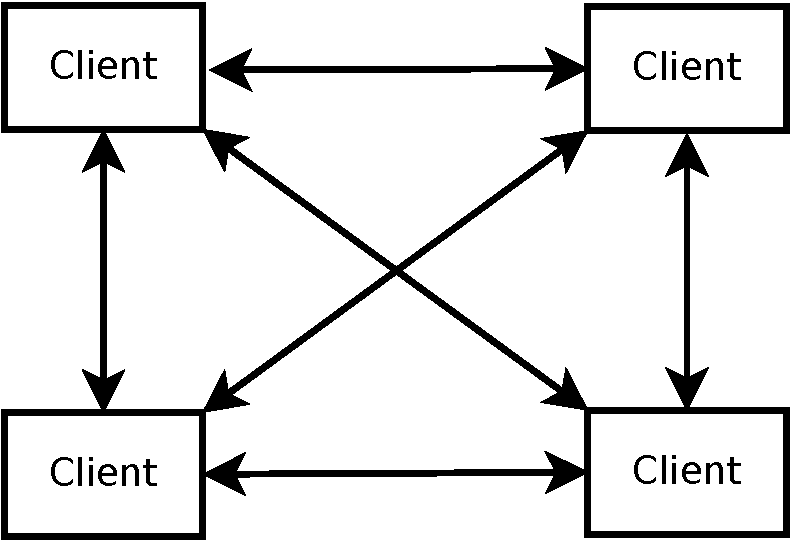
\includegraphics[width=0.48\linewidth]{../images/p2p-model-crop.pdf} &
		%trim=l b r t
		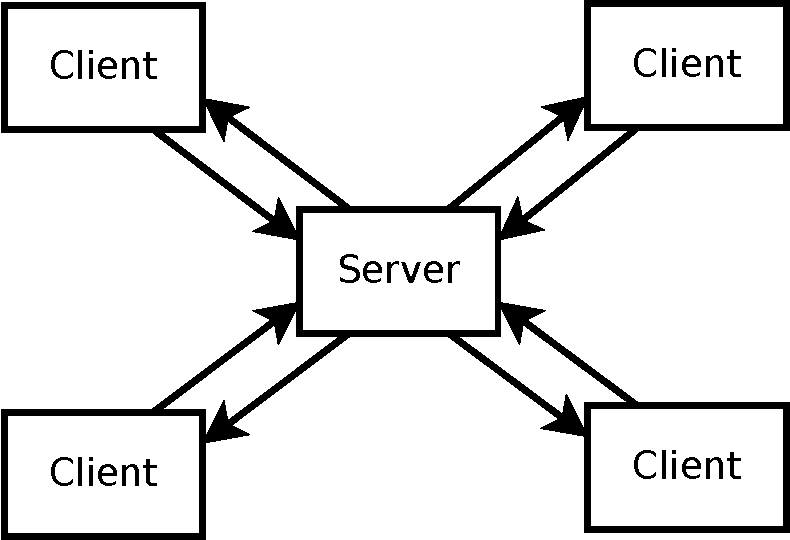
\includegraphics[width=0.48\linewidth]{../images/client-server-model-crop.pdf} \\
		(a) & (b)
	\end{tabular}

	\caption{\label{figure:p2p-vs-ClientServer} Two mutiplayer game networking models. The model on the left (a) is a \ptoP model where every client sends updates directly to ever other client in the game. The second model (b) is a \clientServer model. In this model all of the clients send updates to the server and the server send updates out to the clients.}
	\end{figure}
	
	We choose to base our work off of the \clientServer model for a number of reasons
	\begin{enumerate}
		\item The \clientServer model tends to have less latency
		\item The \clientServer model supports clients joining mid game
		\item The \clientServer model is less susceptible to cheating/malicious clients.
	\end{enumerate}
	
	As in most multiplayer game networking systems asynchronous communication is used. This is necessary to preserve the real-time nature of the game. Packet loss is considered not significant as a new packet with more up-to-date information will be sent soon after the lost packet.
	
\subsection{The Client}

	The client locally simulates its own version of the game. To support this the client needs to keep a list of the other clients in the game and the most recent location of each client. This information will be stored in a map. At every simulation timestep in the game the client will send a position update to the server.
	
\subsection{The Server}

	The server simulates its own version of the game. The server is not used just to reduce message passing but also to act as an authority over the client to prevent cheating/malicious clients from propagating false information.
	
	In the simulation loop for the server a number of actions occur
	\begin{enumerate}
		\item The server's local copy of the clients locations are updated
		\item The server processes any events in its event queue
		\item If the events are valid the server is updated and the result is broadcast to the clients
	\end{enumerate}
	On a different thread
	\begin{enumerate}
		\item The server accepts position updates from clients
		\item The server verifies these updates to be valid
		\item The server broadcasts valid client updates
		\item the server accepts event messages and puts them in a queue for processing on the next timestep
	\end{enumerate}
	
	This way the server keeps the true state of the game and informs the clients of updates to the server's state. To perform these operations the server needs to have state for the currently active clients and its own version of the game state.

\subsection{The Game}

	We will simulate a very basic game to use as our state to synchronize. 
	The game has two possible actions \move{\agent}{\position} and \fire{$\agent_{i}$}{$\agent_{j}$}.
\begin{enumerate}
	\item Common multiplayer model
		\begin{enumerate}
		\item latency minimization
		\item distributed state synchronization
		\item Avoiding cheating
	\end{enumerate}
	\item How Clients work
	\begin{enumerate}
		\item Client data
		\item Client messaging
	\end{enumerate}

	\item How the server works
	\begin{enumerate}
		\item Server data
		\item Server messaging
	\end{enumerate}
	\item The Game
	\begin{enumerate}
		\item The game keeps a natural vector clock (simulation time)
		\item Game data
		\item Game events/messaging
		\begin{enumerate}
			\item move
			\item fire
		\end{enumerate}
	\end{enumerate}
	\item Distributing the game
	\begin{enumerate}
		\item {Two server example}
		\item {Many server example}
		\begin{enumerate}
			\item The best serves can be choosen between two clients and most likely it will be the server on one of the two clients.
		\end{enumerate}
	\end{enumerate}
\end{enumerate}
\todo{Up this point we have really only solved fault tolerance. If we want to solve some scalability issue we will need to provide spatial partitioning of the Game world.}

